This section reports full-Drake multibody simulation results across $N \in \{3, 5, 7\}$ with abrupt cable-snap faults. All results use the Drake~\cite{drake2024} plant at $\Delta t_{\mathrm{sim}} = 0.2$~ms with bead-chain cable dynamics and $30$~s figure-eight trajectories. Specifically, each physical cable is modeled as a chain of 8 point-mass beads connected by 9 tension-only spring-damper segments. This high-fidelity representation captures realistic elastic tension surges and slack behavior during abrupt severing faults, distinguishing it from the simplified scalar topology used for the analytical bounds.

\begin{remark}[System Under Test]\label{rem:system_under_test}
The full-Drake results use Layers~1--2 of the GPAC hierarchy (PID position control with gravity/cable-tension feedforward and geometric $\SOthree$ attitude control). Layer~3 (CL mass estimator), Layer~4 (ESO), and the $\mathcal{L}_1$ adaptive path are \textbf{disabled}. The CBF safety filter is \textbf{disabled}. Sensor state is \textbf{plant-state-direct} (ESKF disabled). Wind disturbance is \textbf{disabled} in the ideal runs; ESKF and Dryden wind are \textbf{active} in the sensor-realistic evaluation.
\end{remark}

The per-agent controller uses PID position feedback ($k_p = 8.0$, $k_d = 8.0$, $k_i = 0.15$), gravity feedforward, cable-tension feedforward ($\kappa_T = 0.5$), anti-swing damping ($k_{\mathrm{sw}} = 0.5$), and geometric $\SOthree$ attitude tracking---all N-agnostic by construction. Three canonical scenarios of increasing difficulty are evaluated:

\begin{enumerate}[label=(\roman*),nosep]
  \item \emph{Three drones, single fault:} $N = 3$, cable lengths $[1.00, 1.08, 1.16]$~m. Cable~$0$ severed at $t_f = 7.0$~s. Post-fault: $2$ agents, $50\%$ load-share increase.
  \item \emph{Five drones, two cascading faults:} $N = 5$, cable lengths $[1.00, 1.05, 1.10, 1.14, 1.18]$~m. Cable~$1$ at $7.0$~s, cable~$3$ at $12.0$~s. Post-fault: $3$ agents, $67\%$ increase.
  \item \emph{Seven drones, three cascading faults:} $N = 7$, cable lengths $[0.98, 1.01, 1.04, 1.07, 1.10, 1.13, 1.16]$~m. Cables~$1$, $3$, $5$ at $7.0$, $12.0$, $14.0$~s. Post-fault: $4$ agents, $75\%$ increase.
\end{enumerate}

No agent is informed of topology changes except the freed agent itself, which detects its own cable loss via $T_i < T_{\min}$.

% ============================================================
\subsection{Canonical Fault Scenarios}
\label{sec:payload_tracking}
% ============================================================

Table~\ref{tab:scenario_summary} reports payload tracking performance across all canonical scenarios. The ${\sim}35$~cm nominal RMSE reflects PID-only control by design; the full GPAC stack (CL+ESO) would reduce it but would introduce history-dependent terms breaking the topology-invariant structure. The favorable $\rho_{\mathrm{FT}}$ values ($1.26$--$1.39$) partly reflect this choice (larger denominator); with the full stack, $\rho_{\mathrm{FT}}$ increases modestly (Section~\ref{sec:eso_evaluation}). The absolute post-fault RMSE ($44$--$49$~cm) is the operationally relevant quantity: it is about three payload radii and roughly $40\%$ of a nominal $1.0$--$1.2$~m cable length, so the controller preserves transport continuity rather than precision placement. Empirical $\rho_{\mathrm{FT}}^{\mathrm{emp}}$ falls below the conservative bound $N/(N{-}k)$ from~\eqref{eq:rho_closed_form}, consistent with the transient-aware analysis in Section~\ref{sec:topology_invariance_theorem}. The canonical scenarios themselves confound team size with fault count; the matched single-fault comparison below isolates the team-size effect.

\begin{table}[t]
\centering
\caption{Full-Drake payload tracking performance: nominal and fault scenarios.}
\label{tab:scenario_summary}
\begin{tabular}{lcccc}
\toprule
Scenario & $N$ & Load RMSE & Peak error & $\rho_{\mathrm{FT}}^{\mathrm{emp}}$ \\
         &     & [cm]      & [cm]       &  \\
\midrule
Three drones, no fault  & 3 & 35.12 & 110.57 & --- \\
Five drones, no fault   & 5 & 34.84 & 110.10 & --- \\
Seven drones, no fault  & 7 & 34.70 & 108.65 & --- \\
\midrule
Three drones, 1~fault   & 3 & 48.84 & 107.44 & 1.39 \\
Five drones, 2~faults   & 5 & 46.37 & 112.30 & 1.33 \\
Seven drones, 3~faults  & 7 & 43.60 & 117.45 & 1.26 \\
\bottomrule
\end{tabular}
\end{table}

The canonical scenarios suggest that average payload RMSE falls with team size even while the number of faults increases: the $N{=}7$ scenario absorbs three cascading faults yet achieves $11\%$ lower RMSE than $N{=}3$ with one fault. Peak errors ($107$--$117$~cm) settle within $1$--$2$~s (Figs.~\ref{fig:tracking_errors_all},~\ref{fig:load_error_overlay}), and each snap produces a bounded reconfiguration rather than loss of transport (Fig.~\ref{fig:scenario_seven}). The matched single-fault comparison below shows that the same trend persists once the fault schedule is held fixed.

\begin{figure*}

    \centering
    \begin{subfigure}[t]{0.24\textwidth}
    \centering
    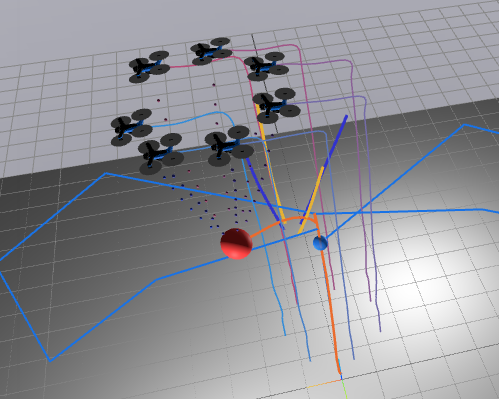
\includegraphics[width=\textwidth]{./Figures/full_drake/seven_drones/7-drones_0.png}
    \caption{}
    \end{subfigure}
    \hfill
    \begin{subfigure}[t]{0.24\textwidth}
    \centering
      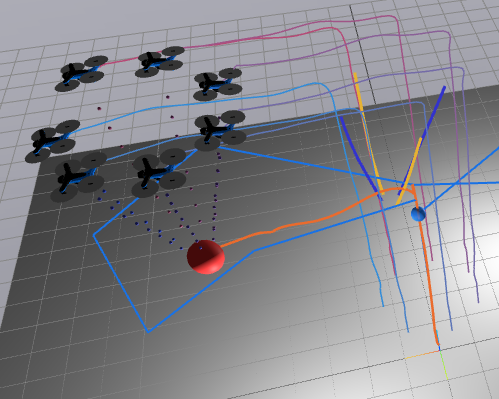
\includegraphics[width=\textwidth]{./Figures/full_drake/seven_drones/7-drones_1.png}
      \caption{}
    \end{subfigure}
    \hfill
    \begin{subfigure}[t]{0.24\textwidth}
    \centering
      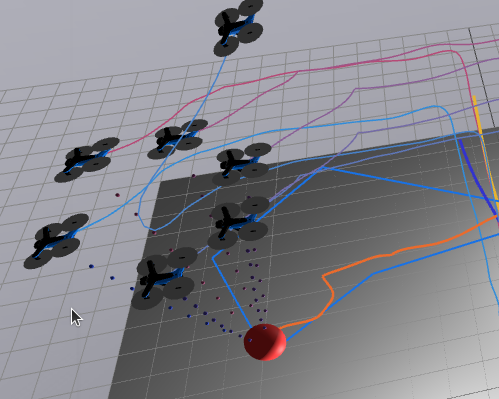
\includegraphics[width=\textwidth]{./Figures/full_drake/seven_drones/7-drones_2.png}
      \caption{}
    \end{subfigure}
    \begin{subfigure}[t]{0.24\textwidth}
    \centering
      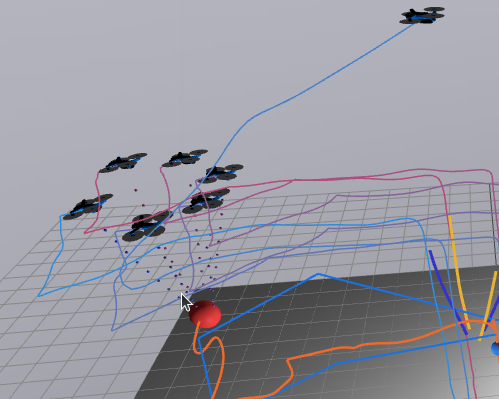
\includegraphics[width=\textwidth]{./Figures/full_drake/seven_drones/7-drones_3.png}
      \caption{}
    \end{subfigure}

     \vspace{0.5em} % Space between rows

     % Row 2
     \begin{subfigure}[b]{0.24\textwidth}
        \centering
        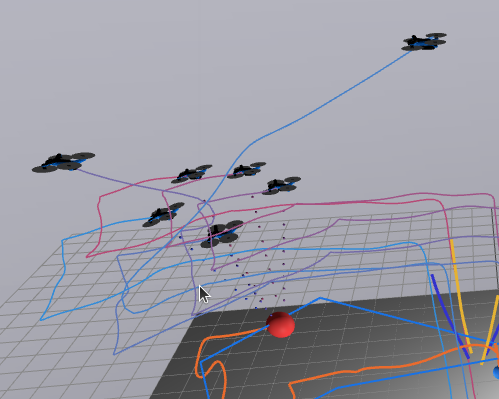
\includegraphics[width=\textwidth]{./Figures/full_drake/seven_drones/7-drones_4.png}
        \caption{}
     \end{subfigure}
     \hfill
      \begin{subfigure}[b]{0.24\textwidth}
        \centering
        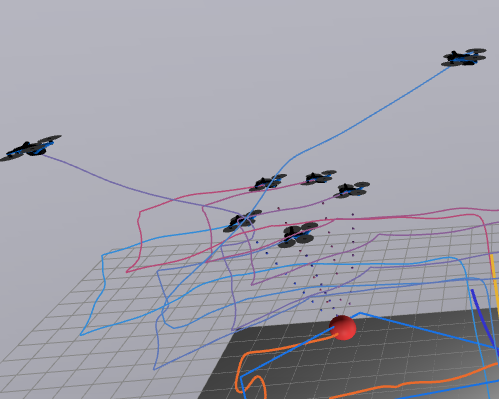
\includegraphics[width=\textwidth]{./Figures/full_drake/seven_drones/7-drones_5.png}
        \caption{}
     \end{subfigure}
      \begin{subfigure}[b]{0.24\textwidth}
        \centering
        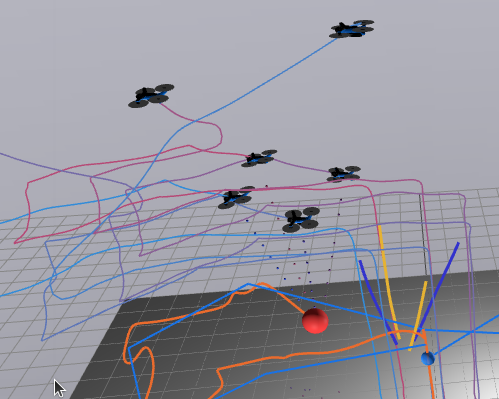
\includegraphics[width=\textwidth]{./Figures/full_drake/seven_drones/7-drones_6.png}
        \caption{}
     \end{subfigure}
      \begin{subfigure}[b]{0.24\textwidth}
        \centering
        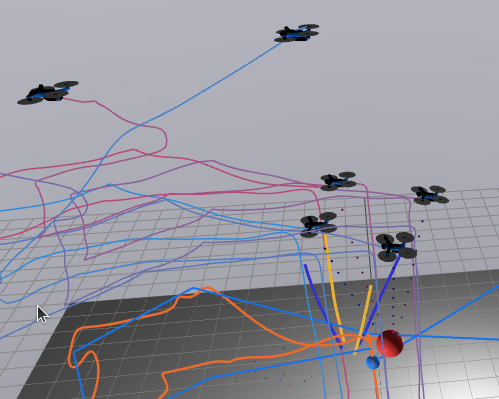
\includegraphics[width=\textwidth]{./Figures/full_drake/seven_drones/7-drones_7.png}
        \caption{}
     \end{subfigure}

  \caption{Seven-drone scenario ($N = 7$, cables~$1$, $3$, $5$ at $7.0$, $12.0$, $14.0$~s). (a) at the start of the mission. (b) about $1$~s before first fault. (c) about  $1$~s after first fault. (d) about $1$~s before second fault. (e) about $1$~s after second fault. (f) about $1$~s before third fault. (g) about $1$~s after third fault. (h) Settled after all faults: $Q_0$, $Q_2$, $Q_4$, $Q_6$ remain.}
  \label{fig:scenario_seven}
\end{figure*}

Cable tensions (Fig.~\ref{fig:tensions_all}) confirm the load-redistribution mechanism: when a cable snaps, remaining cables exhibit a tension surge as they absorb the redistributed load. The freed agent detects the fault via $T_i < T_{\min}$ within the $0.12$~s debounce window and initiates escape. Detection latency is consistent across all six fault events (Table~\ref{tab:fault_detection}), with all freed agents reaching $2.06$--$4.73$~m final separation. Progressive tension oscillation growth reflects cable pendulum near-resonance (${\sim}2$~s period vs.\ ${\sim}3$~s trajectory corner interval); all tensions remain positive, with peaks (${\sim}25$~N) well within limits ($f_{\max} = 150$~N).

\begin{figure}[t]
\centering
\begin{subfigure}[t]{\columnwidth}
  \centering
  
\includegraphics[width=\columnwidth]{./Figures/full_drake/three_drones/payload_tracking_error.png}
  \caption{$N = 3$, single fault at $t = 7.0$~s.}
  \label{fig:tracking_error_three}
\end{subfigure}\\[2pt]
\begin{subfigure}[t]{\columnwidth}
  \centering
  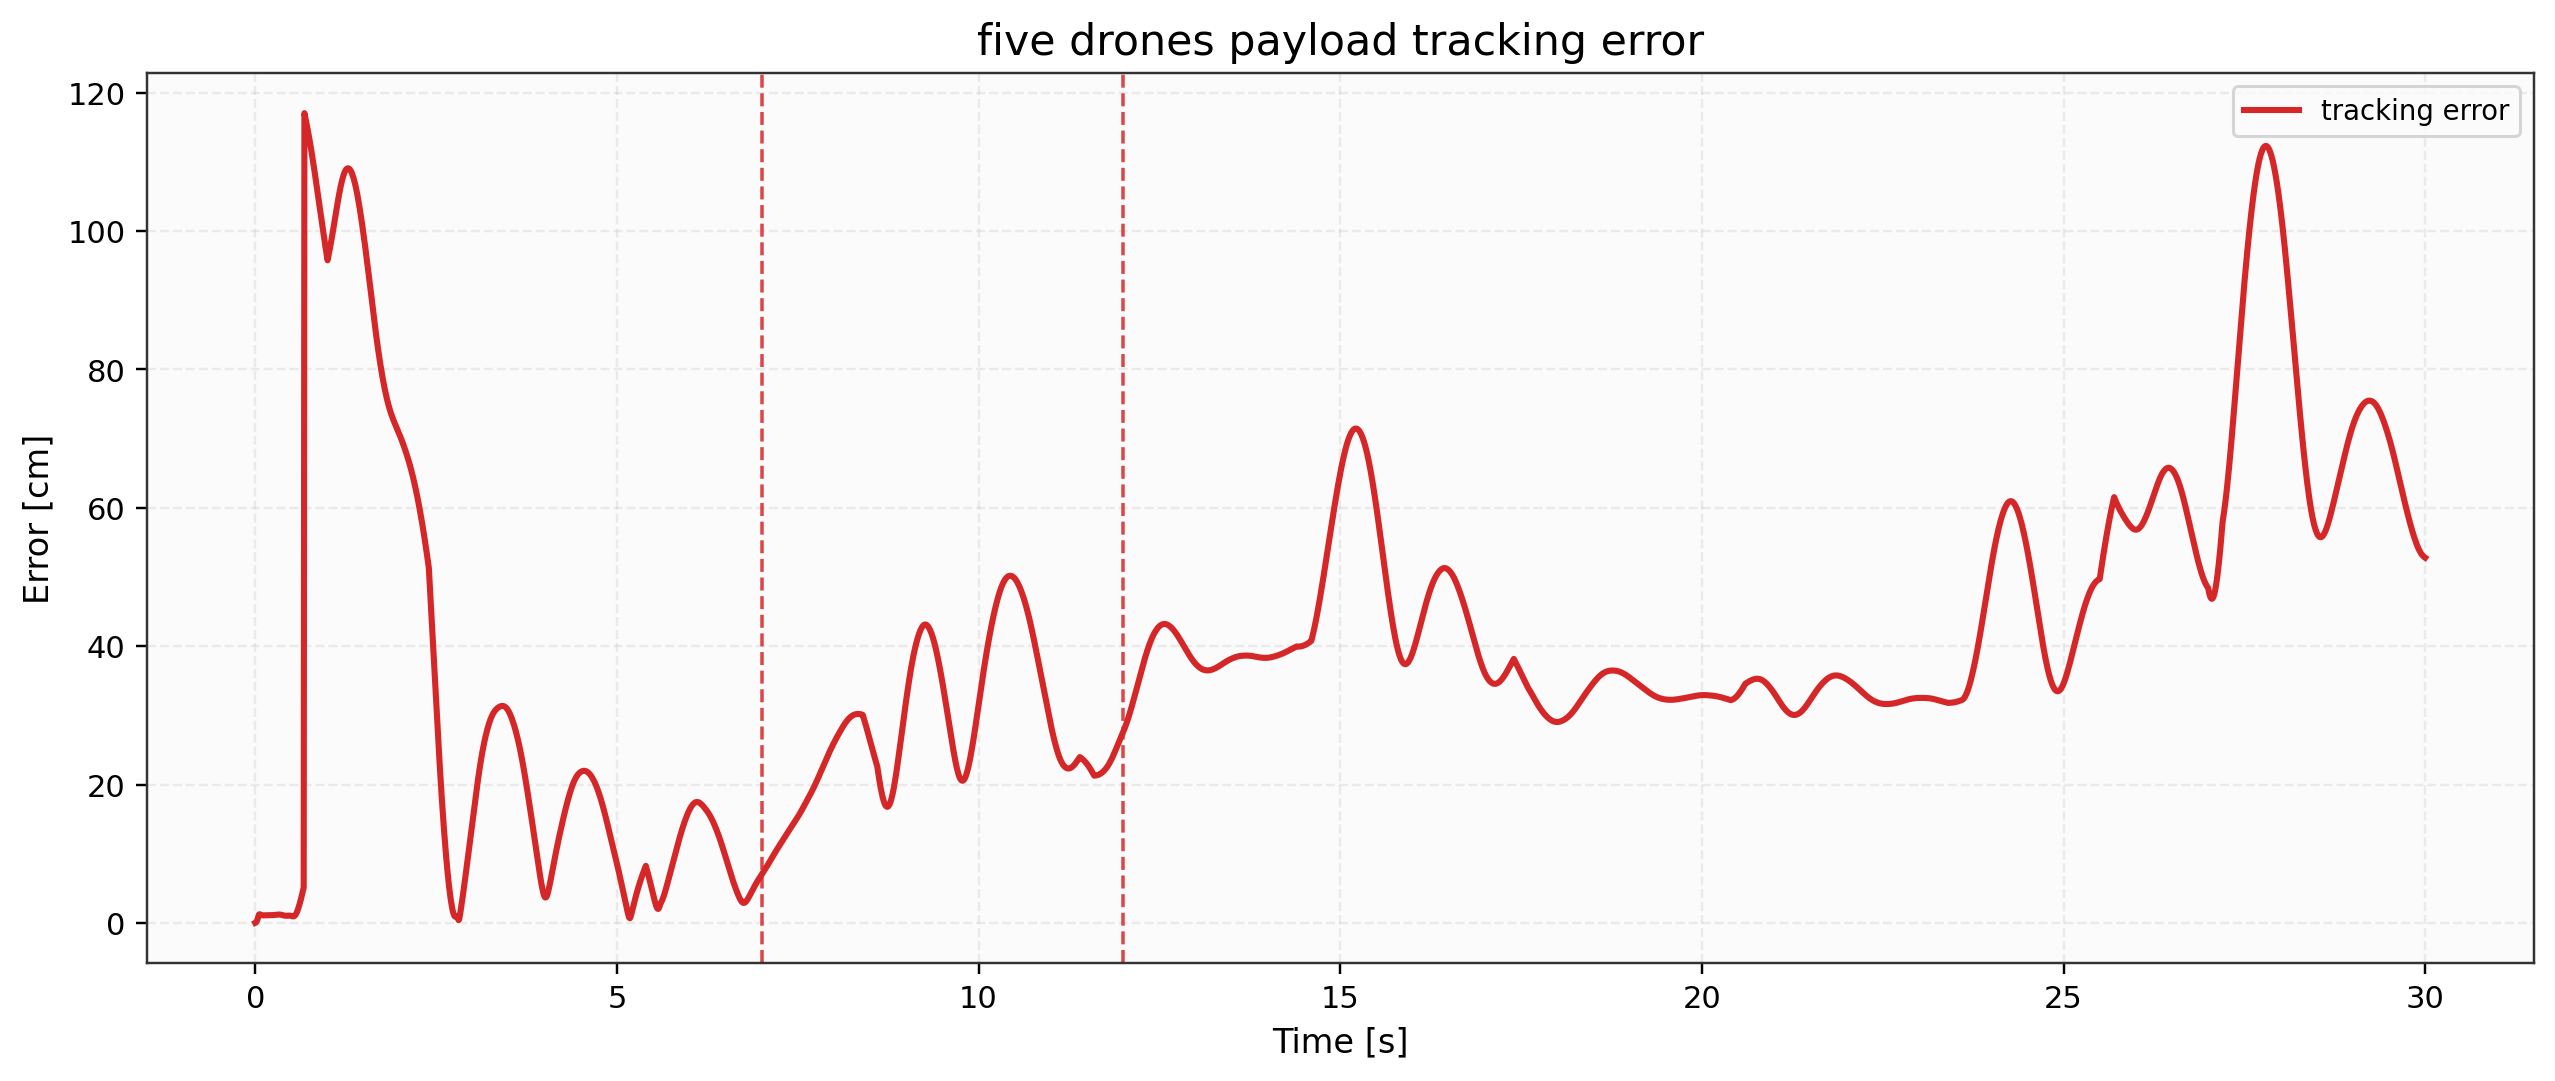
\includegraphics[width=\columnwidth]{./Figures/full_drake/five_drones/payload_tracking_error.png}
  \caption{$N = 5$, two cascading faults.}
  \label{fig:tracking_error_five}
\end{subfigure}\\[2pt]
\begin{subfigure}[t]{\columnwidth}
  \centering
  
\includegraphics[width=\columnwidth]{./Figures/full_drake/seven_drones/payload_tracking_error.png}
  \caption{$N = 7$, three cascading faults within $7$~s.}
  \label{fig:tracking_error_seven}
\end{subfigure}
\caption{Payload tracking error across scenarios. Each fault produces a bounded transient settling in $1$--$2$~s without explicit fault handling.}
\label{fig:tracking_errors_all}
\end{figure}

\begin{figure}[t]
\centering
\begin{subfigure}[t]{\columnwidth}
  \centering
  
\includegraphics[width=\columnwidth]{./Figures/full_drake/three_drones/cable_tensions.png}
  \caption{$N = 3$. Cable~$0$ snaps at $t = 7.0$~s; cables~$1$, $2$ absorb the load.}
  \label{fig:tensions_three}
\end{subfigure}\\[2pt]
\begin{subfigure}[t]{\columnwidth}
  \centering
  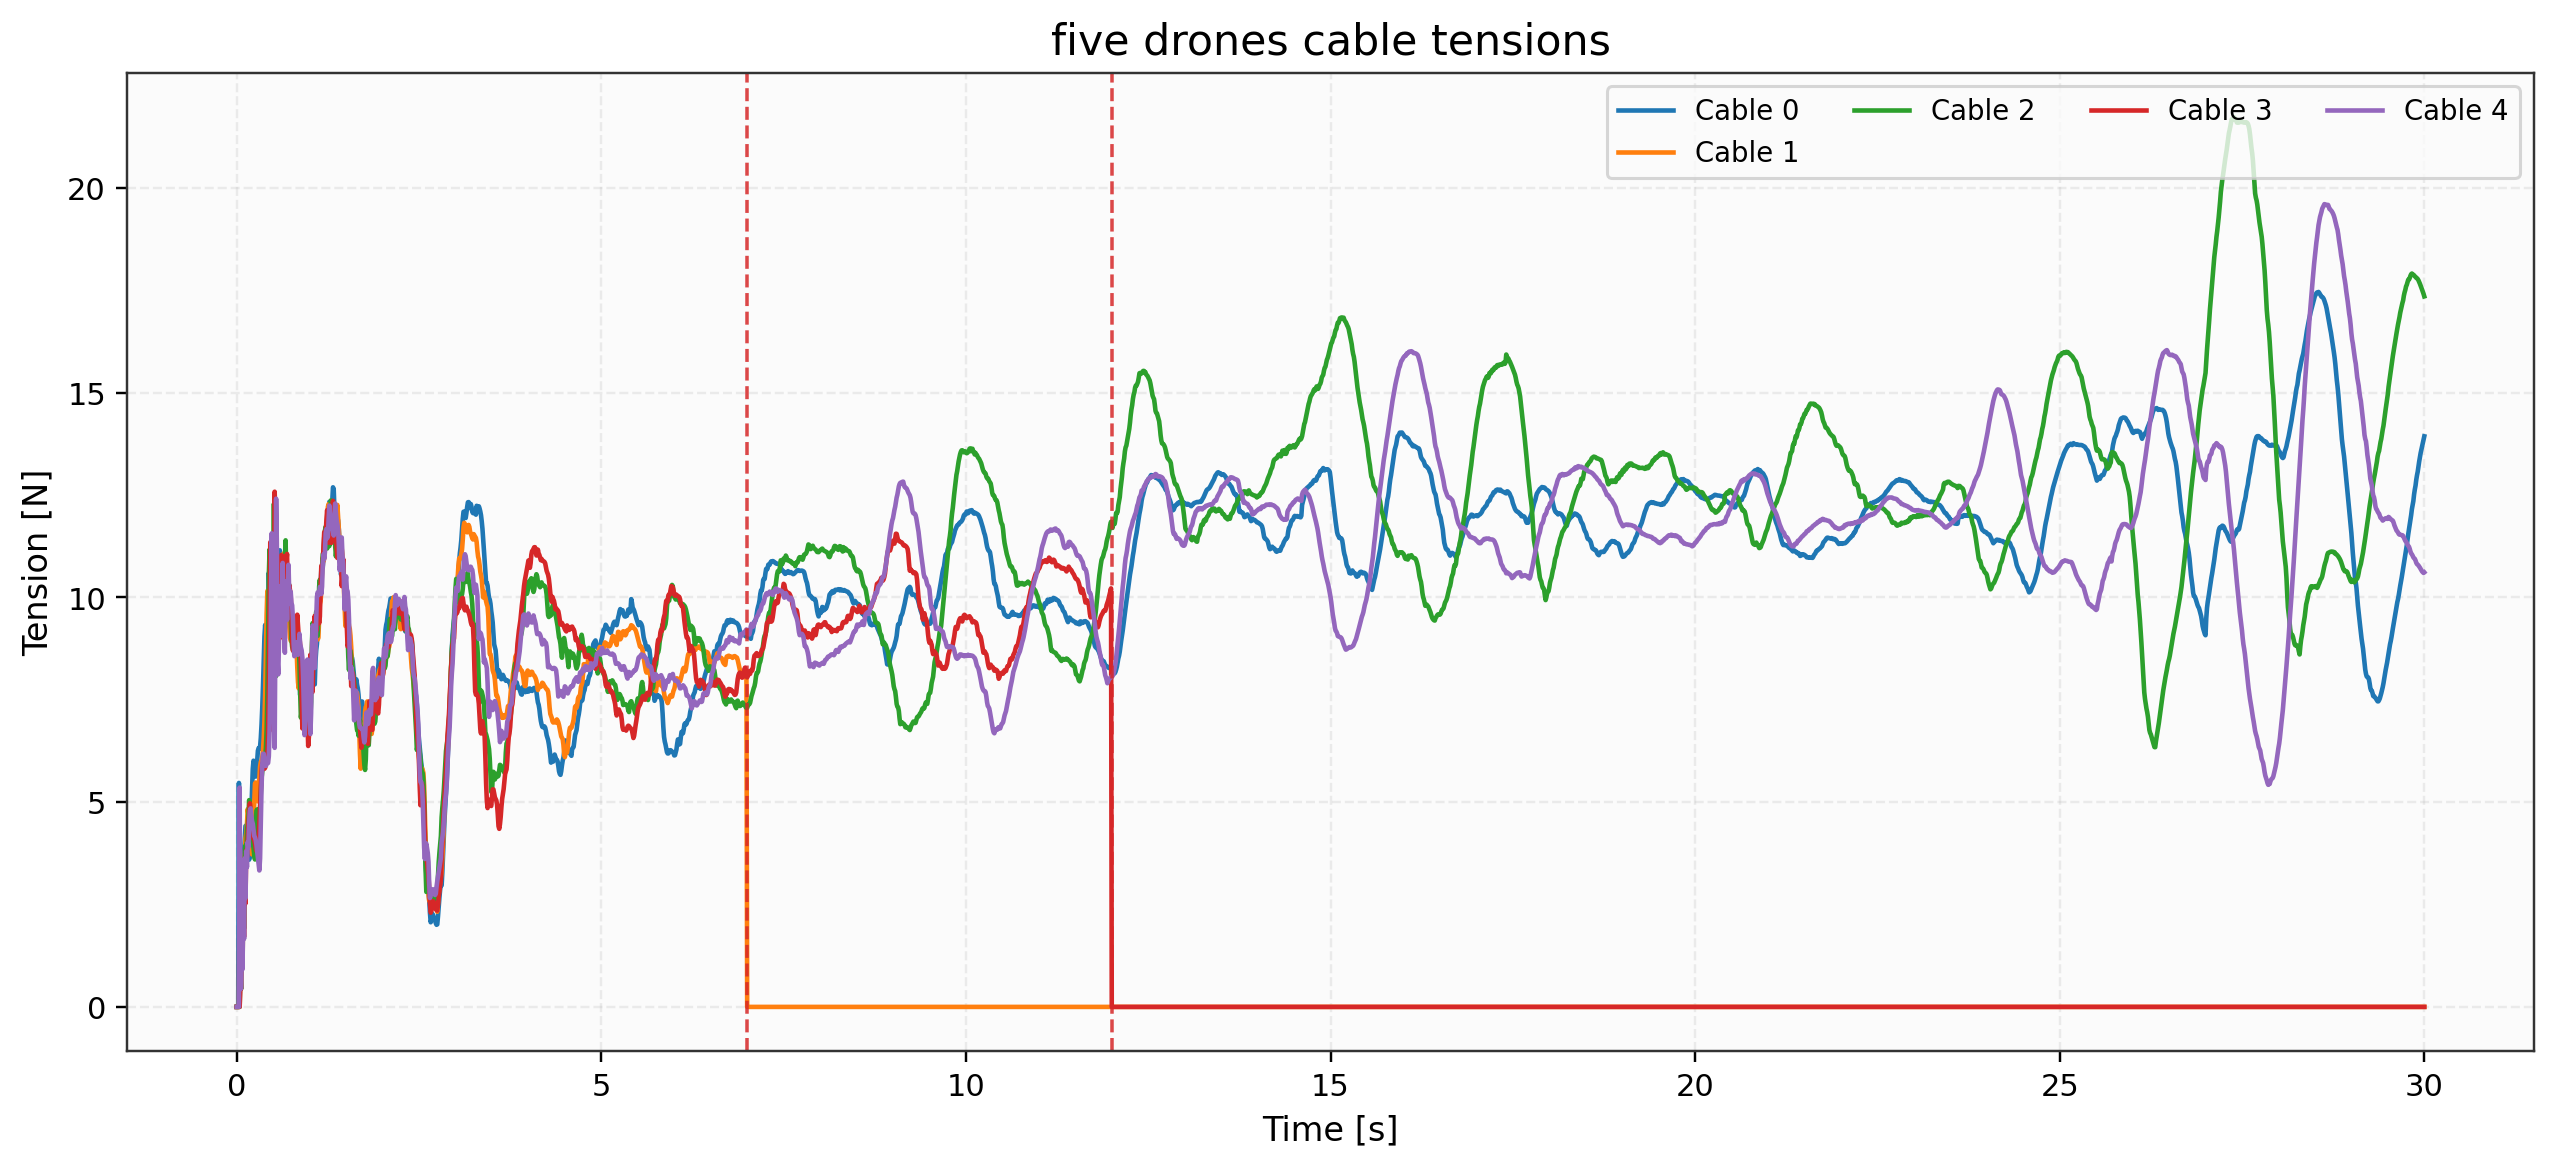
\includegraphics[width=\columnwidth]{./Figures/full_drake/five_drones/cable_tensions.png}
  \caption{$N = 5$. Sequential faults at $7.0$~s and $12.0$~s.}
  \label{fig:tensions_five}
\end{subfigure}\\[2pt]
\begin{subfigure}[t]{\columnwidth}
  \centering
  
\includegraphics[width=\columnwidth]{./Figures/full_drake/seven_drones/cable_tensions.png}
  \caption{$N = 7$. Three sequential faults; four surviving cables remain within limits.}
  \label{fig:tensions_seven}
\end{subfigure}
\caption{Cable tension dynamics across scenarios. Remaining cables exhibit tension surges upon load redistribution; all tensions remain positive and within limits.}
\label{fig:tensions_all}
\end{figure}

\begin{table}[t]
\centering
\caption{Fault detection and freed-agent separation.}
\label{tab:fault_detection}
\begin{tabular}{lcccccc}
\toprule
Scen. & Drone & $t_f$ & Detect. & \multicolumn{3}{c}{Healthy separation [m]} \\
      &       & [s]   & [s]     & at fault & +2\,s & final \\
\midrule
$N{=}3$ & 0 & 7.0  & 0.12 & 0.90 & 1.27 & 2.26 \\
\midrule
$N{=}5$ & 1 & 7.0  & 0.12 & 0.66 & 1.07 & 2.69 \\
        & 3 & 12.0 & 0.12 & 0.65 & 1.96 & 4.68 \\
\midrule
$N{=}7$ & 1 & 7.0  & 0.12 & 0.50 & 1.05 & 2.06 \\
        & 3 & 12.0 & 0.12 & 0.50 & 1.90 & 4.73 \\
        & 5 & 14.0 & 0.12 & 0.50 & 1.69 & 3.82 \\
\bottomrule
\end{tabular}
\end{table}

Vehicle-level dynamics for the most demanding case ($N{=}7$, Fig.~\ref{fig:vehicle_dynamics_seven}) confirm that the GPAC hierarchy maintains stability throughout: after cascading faults, drones~$1$, $3$, $5$ escape while drones~$0$, $2$, $4$, $6$ continue tracking. Formation deviation shows bounded steps at each fault, tilt stays within safe limits, and peak thrust (${\sim}40$~N) remains well below $f_{\max} = 150$~N. The cross-scenario overlay (Fig.~\ref{fig:load_error_overlay}) confirms comparable pre-fault tracking across team sizes, localized $40$--$60$~cm transients per fault event, and stable control even in the $N{=}7$ stress test where the third fault occurs before full recovery from the second. While run-averaged RMSE improves with $N$, terminal error at $t = 30$~s is $42.36$, $52.79$, $54.62$~cm---larger teams improve average tracking but the multi-fault schedules do not produce the smallest end-of-run residual.

\begin{figure*}[t]
\centering
\begin{subfigure}[t]{0.48\textwidth}
  \centering
  
\includegraphics[width=\textwidth]{./Figures/full_drake/seven_drones/xy_trajectories.png}
  \caption{XY trajectories. Drones~$1$, $3$, $5$ depart; $0$, $2$, $4$, $6$ continue.}
  \label{fig:xy_traj_seven}
\end{subfigure}\hfill
\begin{subfigure}[t]{0.48\textwidth}
  \centering
  
\includegraphics[width=\textwidth]{./Figures/full_drake/seven_drones/quad_formation_deviation.png}
  \caption{Formation deviation. Each fault produces a bounded step.}
  \label{fig:formation_seven}
\end{subfigure}\\[4pt]
\begin{subfigure}[t]{0.48\textwidth}
  \centering
  
\includegraphics[width=\textwidth]{./Figures/full_drake/seven_drones/quad_tilt_magnitude.png}
  \caption{Vehicle tilt. Remains within safe limits through all fault transients.}
  \label{fig:tilt_seven}
\end{subfigure}\hfill
\begin{subfigure}[t]{0.48\textwidth}
  \centering
  
\includegraphics[width=\textwidth]{./Figures/full_drake/seven_drones/quad_force_norm.png}
  \caption{Thrust per vehicle. Post-fault ${\sim}40$~N, well below $f_{\max} = 150$~N.}
  \label{fig:force_seven}
\end{subfigure}
\caption{Vehicle-level dynamics for $N = 7$ with three cascading faults. The GPAC hierarchy maintains stability: tilt stays within safe limits and thrust remains well below saturation.}
\label{fig:vehicle_dynamics_seven}
\end{figure*}

\begin{figure}[t]
\centering
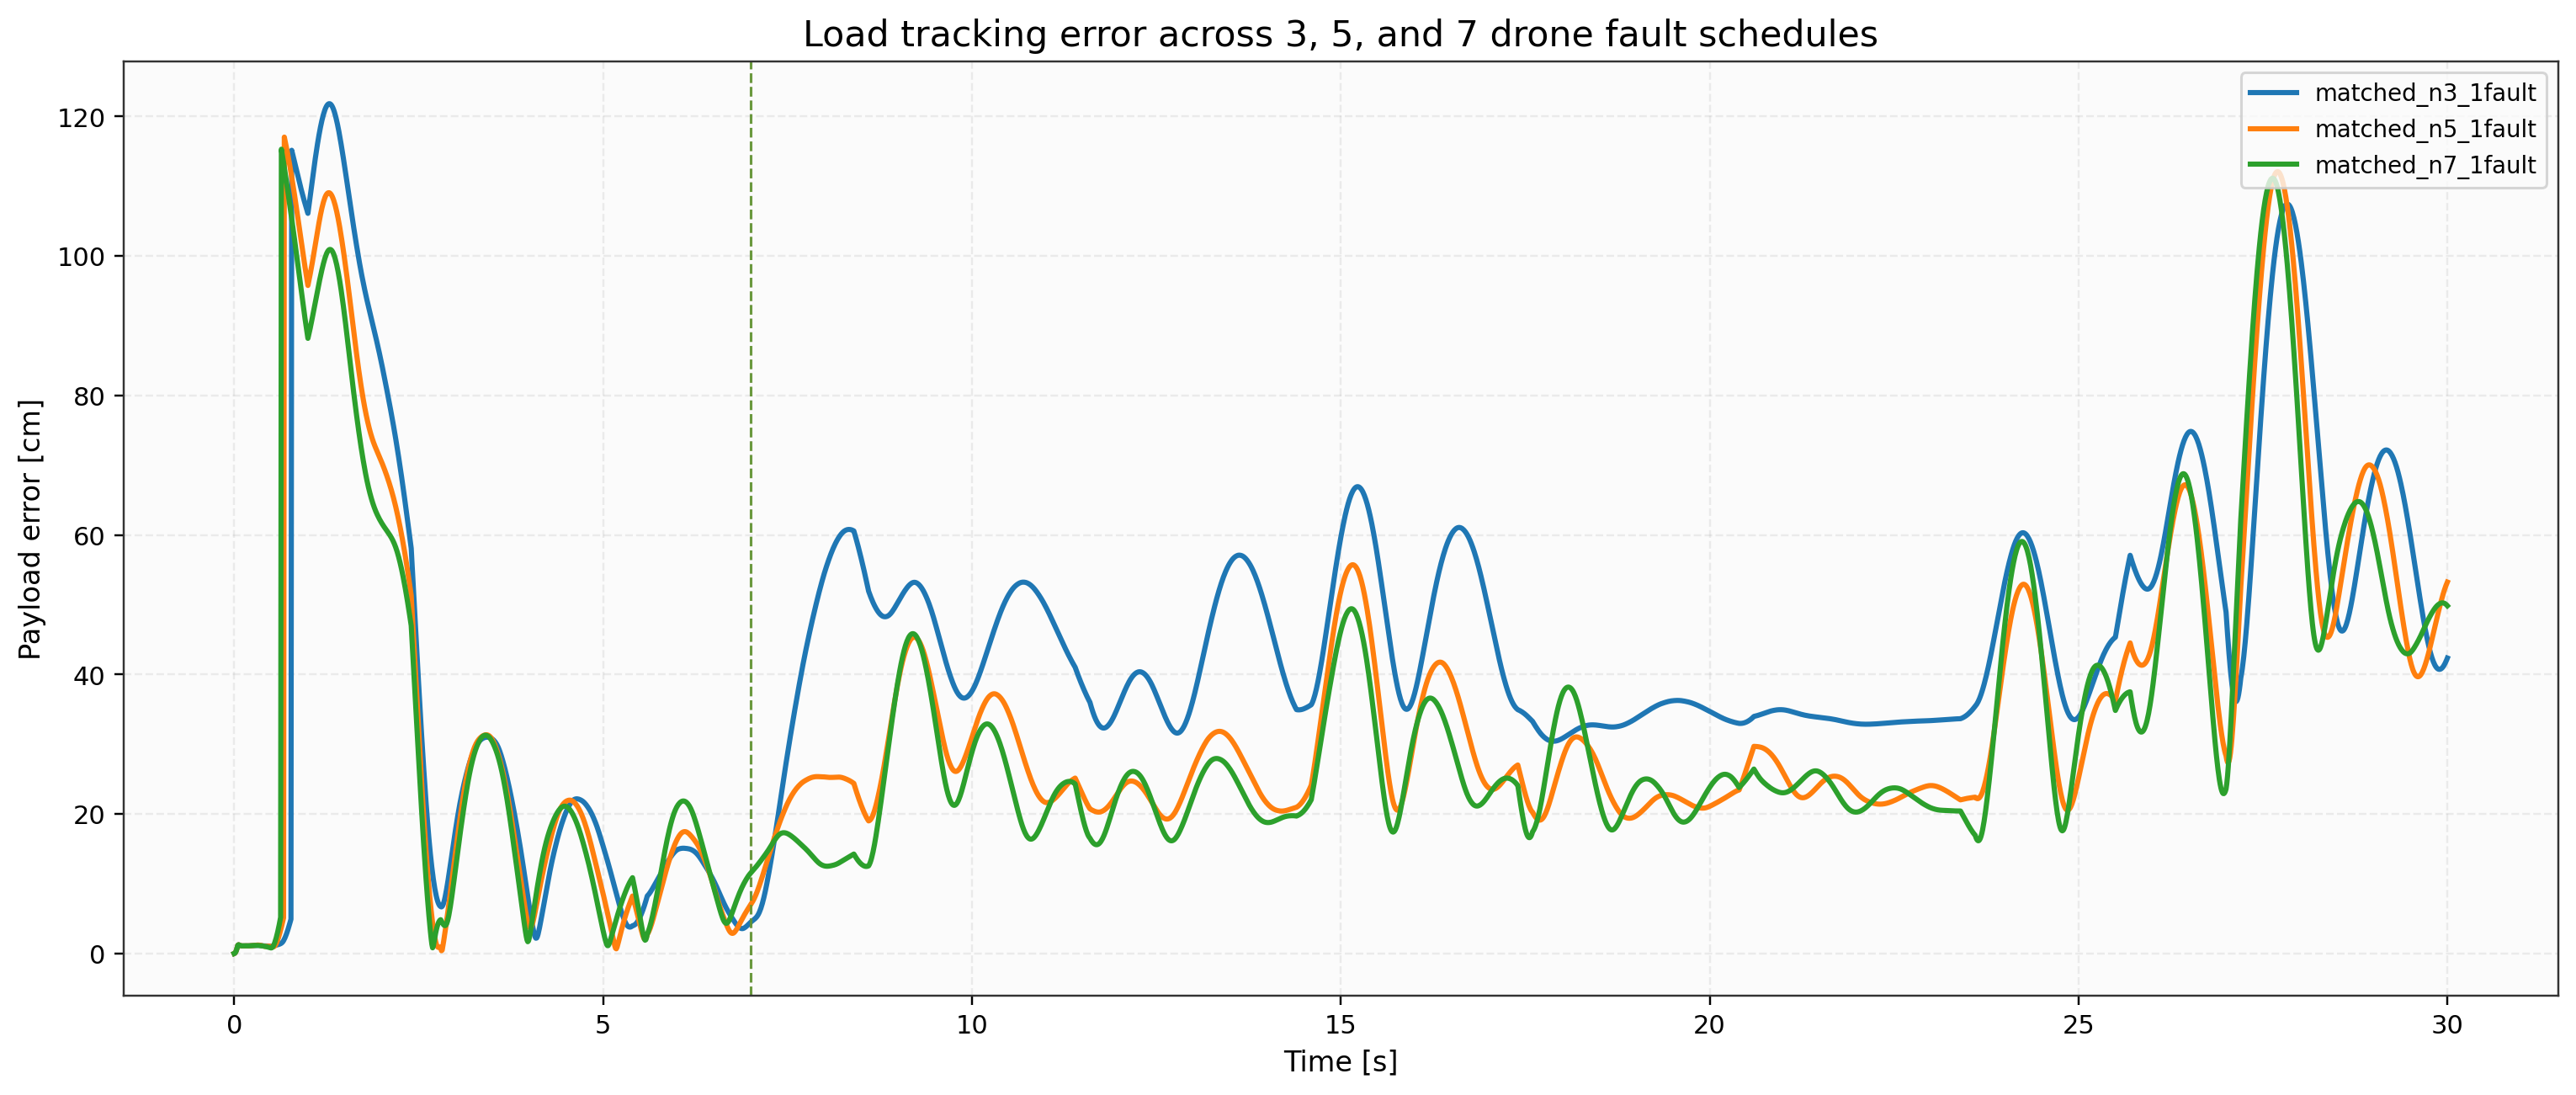
\includegraphics[width=\columnwidth]{./Figures/full_drake/batch_comparison/comparison_load_error_overlay.png}
\caption{Payload tracking error overlay across $N = 3$, $5$, $7$. Fault responses remain localized, settling on $1$--$2$~s timescales.}
\label{fig:load_error_overlay}
\end{figure}

% ============================================================
\subsection{Deconfounding by Team Size, Fault Count, and Thrust Margin}
\label{sec:matched_single_fault}
% ============================================================

The canonical scenarios confound team size with fault count ($1$, $2$, $3$ faults for $N = 3, 5, 7$). Two complementary experiments isolate these variables.

\emph{Matched single-fault comparison.}\label{sec:matched_single_fault_exp}
Applying the \emph{same single-fault event} (cable~$0$ at $t = 7.0$~s) across all three team sizes (Table~\ref{tab:matched_single_fault}), RMSE decreases monotonically: $48.84 \to 40.37 \to 38.38$~cm ($21\%$ improvement from $N{=}3$ to $N{=}7$), confirming that larger capacity ratios translate directly to better tracking. Peak error is nearly constant (${\sim}107$--$112$~cm), set by the cable-snap impulse magnitude. The RMSE improvement comes from faster mid-trajectory recovery, not better final convergence ($N{=}3$ achieves the lowest terminal residual at $42.36$~cm).

\begin{table}[t]
\centering
\caption{Matched single-fault comparison: identical fault event across team sizes.}
\label{tab:matched_single_fault}
\begin{tabular}{lcccc}
\toprule
& $N{=}3$ & $N{=}5$ & $N{=}7$ \\
\midrule
Post-fault capacity ratio & $2/3$ & $4/5$ & $6/7$ \\
Load RMSE [cm]           & 48.84 & 40.37 & 38.38 \\
Peak error [cm]          & 107.44 & 112.09 & 111.15 \\
Final error [cm]         & 42.36 & 53.25 & 49.85 \\
\bottomrule
\end{tabular}
\end{table}

\emph{Fault-count isolation.}\label{sec:fault_count_isolation}
Holding $N{=}7$ constant while varying $k \in \{1, 2, 3\}$ (Table~\ref{tab:fault_count_isolation}), RMSE increases monotonically: $34.70$, $39.39$, $41.29$, $43.60$~cm for $k = 0, 1, 2, 3$. Each additional fault adds ${\sim}2$--$5$~cm RMSE, confirming incremental degradation rather than catastrophic failure. Peak error is highest for $k{=}2$ ($118.21$~cm), likely because the second fault at $t{=}12$~s occurs during an unfavorable trajectory phase.

\begin{table}[t]
\centering
\caption{Fault-count isolation: $N{=}7$ with 1, 2, and 3 faults.}
\label{tab:fault_count_isolation}
\begin{tabular}{lccccc}
\toprule
Faults $k$ & Surviving & Capacity & RMSE & Peak & Final \\
           & agents    & ratio    & [cm] & [cm] & [cm]  \\
\midrule
0 (nominal) & 7 & --- & 34.70 & 108.65 & 43.73 \\
1           & 6 & $6/7$ & 39.39 & 111.26 & 54.43 \\
2           & 5 & $5/7$ & 41.29 & 118.21 & 54.74 \\
3           & 4 & $4/7$ & 43.60 & 117.45 & 54.62 \\
\bottomrule
\end{tabular}
\end{table}

\emph{Thrust-margin verification.}
All scenarios satisfy the thrust-margin condition with capacity ratios $1.75$--$2.33$ (Table~\ref{tab:topology_margin}). Peak tilt during post-fault transients ($15$\textdegree--$25$\textdegree, Fig.~\ref{fig:tilt_seven}) reduces effective vertical thrust by $3$--$9\%$; all scenarios remain well above unity with this correction. A conservative design should use $f_{\max} \cos(\theta_{\max})$ as the effective vertical thrust authority.

\begin{table}[t]
\centering
\caption{Topology-invariance thrust-margin screen.}
\label{tab:topology_margin}
\begin{tabular}{lccccc}
\toprule
Scenario & $N$ & Required & Available & Capacity & Healthy \\
         &     & [N/agent]& [N/agent] & ratio    & fraction \\
\midrule
$N{=}3$, 1~fault & 3 & 29.43 & 51.50 & 1.75 & 0.67 \\
$N{=}5$, 2~faults & 5 & 24.53 & 51.50 & 2.10 & 0.60 \\
$N{=}7$, 3~faults & 7 & 22.07 & 51.50 & 2.33 & 0.57 \\
\bottomrule
\end{tabular}
\end{table}

% ============================================================
\subsection{Mechanism Identification}
\label{sec:tension_ablation}
% ============================================================

Three experiments identify what drives the fault-absorption mechanism and where it breaks.

\emph{Tension feedforward ablation.}\label{sec:fmax_boundary}
Disabling cable-tension feedforward in the most stressed scenario ($N{=}3$, single fault) changes RMSE by only $0.44$~cm ($0.9\%$) and peak error by $0.06$~cm (Table~\ref{tab:tension_ablation}). Varying $\kappa_T$ across $\{0, 0.25, 0.5, 1.0\}$ produces total RMSE variation of $1.55$~cm. This identifies the \emph{primary} fault-absorption mechanism as PID feedback with gravity feedforward---not cable-tension feedforward. Cable-tension feedforward provides a marginal improvement ($0.77$~cm in final error) that is helpful but not essential.

\begin{table}[t]
\centering
\caption{Tension feedforward ablation ($N{=}3$, single fault at $t = 7.0$~s).}
\label{tab:tension_ablation}
\begin{tabular}{lccc}
\toprule
Configuration & RMSE [cm] & Peak [cm] & Final [cm] \\
\midrule
Full feedforward ($\kappa_T = 0.5$) & 48.84 & 107.44 & 42.36 \\
No tension feedforward              & 48.40 & 107.50 & 43.13 \\
\bottomrule
\end{tabular}
\end{table}

\emph{Thrust saturation boundary.}
Sweeping $f_{\max}$ from $150$~N down to $35$~N reveals a sharp phase transition (Table~\ref{tab:fmax_boundary}): for $f_{\max} \in [45, 150]$~N, RMSE stays within $48.8$--$49.1$~cm; at $f_{\max} = 38$~N, it jumps to $236.9$~cm ($4.9\times$ degradation). This coincides with the theoretical minimum:
\begin{equation}\label{eq:fmax_critical}
  f_{\max}^* = \frac{(N \cdot m_Q + m_L) \cdot g}{N - k} + f_{\mathrm{track}} \approx 36.8 + 8 \approx 45\;\text{N},
\end{equation}
where $f_{\mathrm{track}} \approx m_Q \cdot a_{\max} \approx 8$~N accounts for figure-eight tracking demand (matching the observed pre-fault thrust above hover). The default $f_{\max} = 150$~N provides $3\times$ headroom, confirming that the claimed fault tolerance does not depend on aggressive actuator sizing. Below the transition, RMSE is non-monotonic ($236.9$~cm at $38$~N vs.\ $192.1$~cm at $35$~N): the system enters distinct saturation-dominated failure modes where the specific trajectory phase at the fault instant determines which agents saturate and for how long.

\begin{table}[t]
\centering
\caption{Thrust saturation boundary ($N{=}3$, single fault at $t = 7.0$~s).}
\label{tab:fmax_boundary}
\begin{tabular}{lcccc}
\toprule
$f_{\max}$ [N] & $f_{\max}/f_{\mathrm{hover}}$ & RMSE [cm] & Peak [cm] & Final [cm] \\
\midrule
150 & $10.2\times$ & 48.84 & 107.44 & 42.36 \\
 80 & $ 5.4\times$ & 48.84 & 107.44 & 42.36 \\
 60 & $ 4.1\times$ & 48.84 & 107.44 & 42.36 \\
 45 & $ 3.1\times$ & 49.06 & 107.66 & 44.10 \\
 38 & $ 2.6\times$ & 236.92 & 324.97 & 252.35 \\
 35 & $ 2.4\times$ & 192.11 & 250.34 & 179.28 \\
\bottomrule
\end{tabular}
\end{table}

\emph{Controller comparison hierarchy.}\label{sec:baseline_comparison}
To contextualize the passive GPAC approach, three alternative controllers are evaluated on the $N{=}3$ single-fault scenario (Table~\ref{tab:baseline_comparison}): a centralized oracle with perfect post-fault load-share feedforward, a gain-scheduled PID triggered by elevated cable tension, and a threshold-triggered reactive controller that boosts thrust by $+30\%$. The centralized oracle performs comparably to passive GPAC ($49.18$ vs.\ $48.84$~cm, $+0.7\%$), but this should be interpreted narrowly: the oracle only replaces the local cable-tension feedforward term and does not reconfigure geometry, reset the integral state, or alter the trajectory. The absolute difference is $0.34$~cm, smaller than the $0.49$~cm run-to-run standard deviation reported for the same $N{=}3$ fault scenario in Table~\ref{tab:monte_carlo}. The tested detection-based alternatives therefore provide no practically meaningful benefit over the N-agnostic PID-plus-feedforward structure, but this comparison does not rule out stronger centralized policies.

\begin{table}[t]
\centering
\caption{Controller comparison ($N{=}3$, single fault). The centralized oracle uses perfect post-fault load-share feedforward only; it does not alter geometry, trajectory references, or integral states.}
\label{tab:baseline_comparison}
\begin{tabular}{l S[table-format=2.2] S[table-format=3.2] l l}
\toprule
Controller & {RMSE} & {Peak} & Detection & Communication \\
           & [cm] & [cm]       &           &     \\
\midrule
Centralized oracle           & 49.18 & 107.33 & Perfect   & Yes \\
\midrule
Gain-scheduled PID & 48.96 & 106.75 & Threshold & No  \\
($1.5{\times}k_p, 1.25{\times}k_d$) &       &        &           &     \\
\midrule
\textbf{Passive GPAC}     & 48.84 & 107.44 & No        & No  \\
\midrule
Threshold-triggered  & 49.45 & 107.66 & Threshold & No  \\
\bottomrule
\end{tabular}
\end{table}

\emph{ESO-active evaluation.}\label{sec:eso_evaluation}
To assess whether the favorable $\rho_{\mathrm{FT}}$ values are an artifact of the deliberately constrained controller, the ESO disturbance feedforward (Layer~4) is activated in all canonical scenarios (Table~\ref{tab:eso_evaluation}). ESO reduces nominal RMSE by $17$--$18\%$, confirming that PID-only nominal RMSE was inflated by uncompensated cable dynamics. The $\rho_{\mathrm{FT}}$ values increase modestly ($1.37$--$1.46$ vs.\ $1.26$--$1.39$), but absolute post-fault RMSE with ESO ($40$--$46$~cm) is \emph{lower} than PID-only ($44$--$49$~cm)---the $\rho_{\mathrm{FT}}$ increase reflects proportionally larger nominal improvement, not degraded fault tolerance. The topology-invariance property does not hold strictly with ESO active (history dependence); the PID-only evaluation remains the correct test.

\begin{table}[t]
\centering
\caption{ESO-active evaluation: sensitivity of $\rho_{\mathrm{FT}}$ to controller complexity.}
\label{tab:eso_evaluation}
\begin{tabular}{lccccc}
\toprule
& \multicolumn{2}{c}{RMSE [cm]} & \multicolumn{2}{c}{$\rho_{\mathrm{FT}}$} \\
Scenario & Nominal & Fault & ESO & PID-only \\
\midrule
$N{=}3$, 1~fault & 28.94 & 40.43 & 1.40 & 1.39 \\
$N{=}5$, 2~faults & 30.50 & 44.59 & 1.46 & 1.33 \\
$N{=}7$, 3~faults & 33.67 & 46.01 & 1.37 & 1.26 \\
\bottomrule
\end{tabular}
\end{table}

% ============================================================
\subsection{Robustness Validation}
\label{sec:sensor_realistic}
% ============================================================

Four complementary evaluations establish robustness beyond the ideal-condition canonical runs.

\emph{Sensor-realistic evaluation.}
Activating the ESKF and Dryden wind model produces moderate, consistent RMSE degradation: $+9.9\%$ for $N{=}3$, $+8.1\%$ for $N{=}5$, and $+10.7\%$ for $N{=}7$ (Table~\ref{tab:sensor_realistic}). All scenarios remain stable with RMSE below $54$~cm, and the uniform ${\sim}10\%$ degradation confirms robustness to sensor noise and wind perturbations. Peak errors increase by $12$--$14$~cm, attributable to wind compounding fault transients and ESKF estimation lag.

\begin{table}[h]
\centering
\caption{Sensor-realistic evaluation}
\label{tab:sensor_realistic}
\begin{tabular}{lccccc}
\toprule
Scenario & \multicolumn{2}{c}{RMSE [cm]} & \multicolumn{2}{c}{Peak error [cm]} \\
         & Ideal & ESKF+wind & Ideal & ESKF+wind \\
\midrule
$N{=}3$, 1~fault   & 48.84 & 53.68 & 107.44 & 119.14 \\
$N{=}5$, 2~faults  & 46.37 & 50.14 & 112.30 & 125.17 \\
$N{=}7$, 3~faults  & 43.60 & 48.28 & 117.45 & 131.56 \\
\bottomrule
\end{tabular}
\end{table}

\emph{Monte Carlo validation.}\label{sec:monte_carlo}
A campaign of $N_{\mathrm{MC}} = 30$ runs per scenario randomizes cable lengths (${\pm}5\%$), wind seeds, and simulation seeds while using the same fixed fault schedule. Standard deviations of $0.49$--$1.34$~cm (Table~\ref{tab:monte_carlo}) confirm robustness to plant-parameter variation ($<3\%$ RMSE variation across $30$ runs). MC means are consistent with the deterministic values in Table~\ref{tab:scenario_summary} (within $1\%$), confirming representativeness. The 95th-percentile peak errors ($108$--$120$~cm) remain well within thrust-margin headroom.

\begin{table}[t]
\centering
\caption{Monte Carlo results (mean $\pm$ std over $N_{\mathrm{MC}}$ runs).}
\label{tab:monte_carlo}
\begingroup
\setlength{\tabcolsep}{3.5pt}
\renewcommand{\arraystretch}{0.96}
\footnotesize
\begin{tabular}{@{}lcccc@{}}
\toprule
Scenario & $N_{\mathrm{MC}}$ & RMSE [cm] & Peak [cm] & 95th pctl. \\
         &                    & mean $\pm$ std & mean $\pm$ std & peak [cm] \\
\midrule
$N{=}3$, 1 fault   & 30 & $48.84 \pm 0.49$ & $107.28 \pm 0.47$ & 107.85 \\
$N{=}5$, 2 faults  & 30 & $46.40 \pm 0.49$ & $112.23 \pm 1.07$ & 113.89 \\
$N{=}7$, 3 faults  & 30 & $43.95 \pm 1.34$ & $117.55 \pm 1.37$ & 119.84 \\
$N{=}3$, ESKF+wind & 30 & $53.62 \pm 0.83$ & $118.83 \pm 0.91$ & 120.19 \\
\bottomrule
\end{tabular}
\endgroup
\end{table}

\emph{Broadened Monte Carlo.}\label{sec:broadened_mc}
A broadened campaign additionally randomizes payload mass (${\pm}10\%$), PID gains (${\pm}10\%$), and fault timing (${\pm}2$~s). In $5$ runs for $N{=}3$, broadened RMSE is $48.04 \pm 1.29$~cm (vs.\ narrow MC $48.84 \pm 0.49$~cm): standard deviation increases ${\sim}2.6\times$ but all runs remain stable. Because this broadened campaign contains only five trials, it is interpreted here as exploratory evidence of robustness to simultaneous plant-parameter variation rather than as the same statistical tier as Table~\ref{tab:monte_carlo}.

\emph{Trajectory generalization.}\label{sec:trajectory_generalization}
Testing across hover, point-to-point, and figure-eight references in the supplementary material confirms that the fault-absorption mechanism operates consistently: RMSE decreases with team size and remains bounded across all trajectory types. Hover RMSE is $19\%$ lower than figure-eight ($39.75$ vs.\ $48.84$~cm for $N{=}3$), confirming that the figure-eight amplifies post-fault error through cable-pendulum near-resonance.

% ============================================================
\subsection{Cable Discretization Sensitivity}
\label{sec:bead_discretization}
% ============================================================

The bead-chain cable model discretizes each continuous cable into $n_b$ point-mass beads connected by $(n_b{+}1)$ tension-only spring-damper segments. All preceding results use $n_b{=}8$. A dedicated sweep over $n_b \in \{2, 4, 8, 12, 16\}$ in the $N{=}5$ cascading-fault scenario kept cable-level stiffness and damping invariant while varying spatial resolution. Across the full range, the first-fault peak error changed by only $0.3$~cm ($31.5$--$31.8$~cm), the second-fault peak by $0.2$~cm ($43.2$--$43.4$~cm), the whole-run RMSE by $0.1$~cm ($43.1$--$43.2$~cm), and the recovery times remained $4.09$~s and $3.67$~s for the two faults. The main fault-tolerant transport conclusion is therefore insensitive to cable discretization over the tested range, and the $n_b{=}8$ baseline remains the practical choice.

